
% \subsection{ Makrozyklus Schritt 1: Zustandssimulation und Datengenerierung}

Die Generierung der Schaltungszustände, die als Input für den Lernprozess dienen, erfolgt mittels einer Zufallsfunktion. In der realen Welt erfolgen Zustandsübergänge in einer physischen Schaltung in langen Zeitintervallen, was eine direkte Simulation unpraktisch macht. Deshalb greifen wir auf eine alternative Methode zurück:

\begin{itemize}
    \item Initial wird über eine Gleichverteilung ein Degenerationszustand der Schaltung simuliert. Die zufällige Auswahl dieser Zustände geschieht innerhalb festgelegter Grenzen, um eine Vielfalt an möglichen Zuständen zu gewährleisten.
	\item Der simulierte Zustand wird durch einen Satz von Kapazitäts- und Induktivitätswerten dargestellt. Diese Werte werden durch den "Würfel" im System visualisiert \ref{fig:state_generation}, wobei die Pfeile vom Würfel zu den Zustandsvariablen C und L diesen Prozess der zufälligen Zustandsgenerierung abbilden.
\end{itemize}

In diesem Projekt werden exemplarische Einstellungen für die Zustandsgenerierung verwendet, die eine Annäherung an realitätsnahe Bedingungen darstellen. Bei einer Überführung in praktische Anwendungen würden diese Einstellungen so angepasst, dass sie mit den in der Realität verifizierten Werten übereinstimmen. Die aktuellen Grenzwerte für die Zustandsgenerierung sind wie folgt definiert:

\begin{itemize}
    \item Untergrenze: \( \text{Induktivität} = 5.0 \times 10^{-4} \), \( \text{Kapazität} = 1.0 \times 10^{-6} \)
    \item Obergrenze: \( \text{Induktivität} = 5.0 \times 10^{-2} \), \( \text{Kapazität} = 1.0 \times 10^{-4} \)
\end{itemize}

\begin{figure}[htbp]
\centering
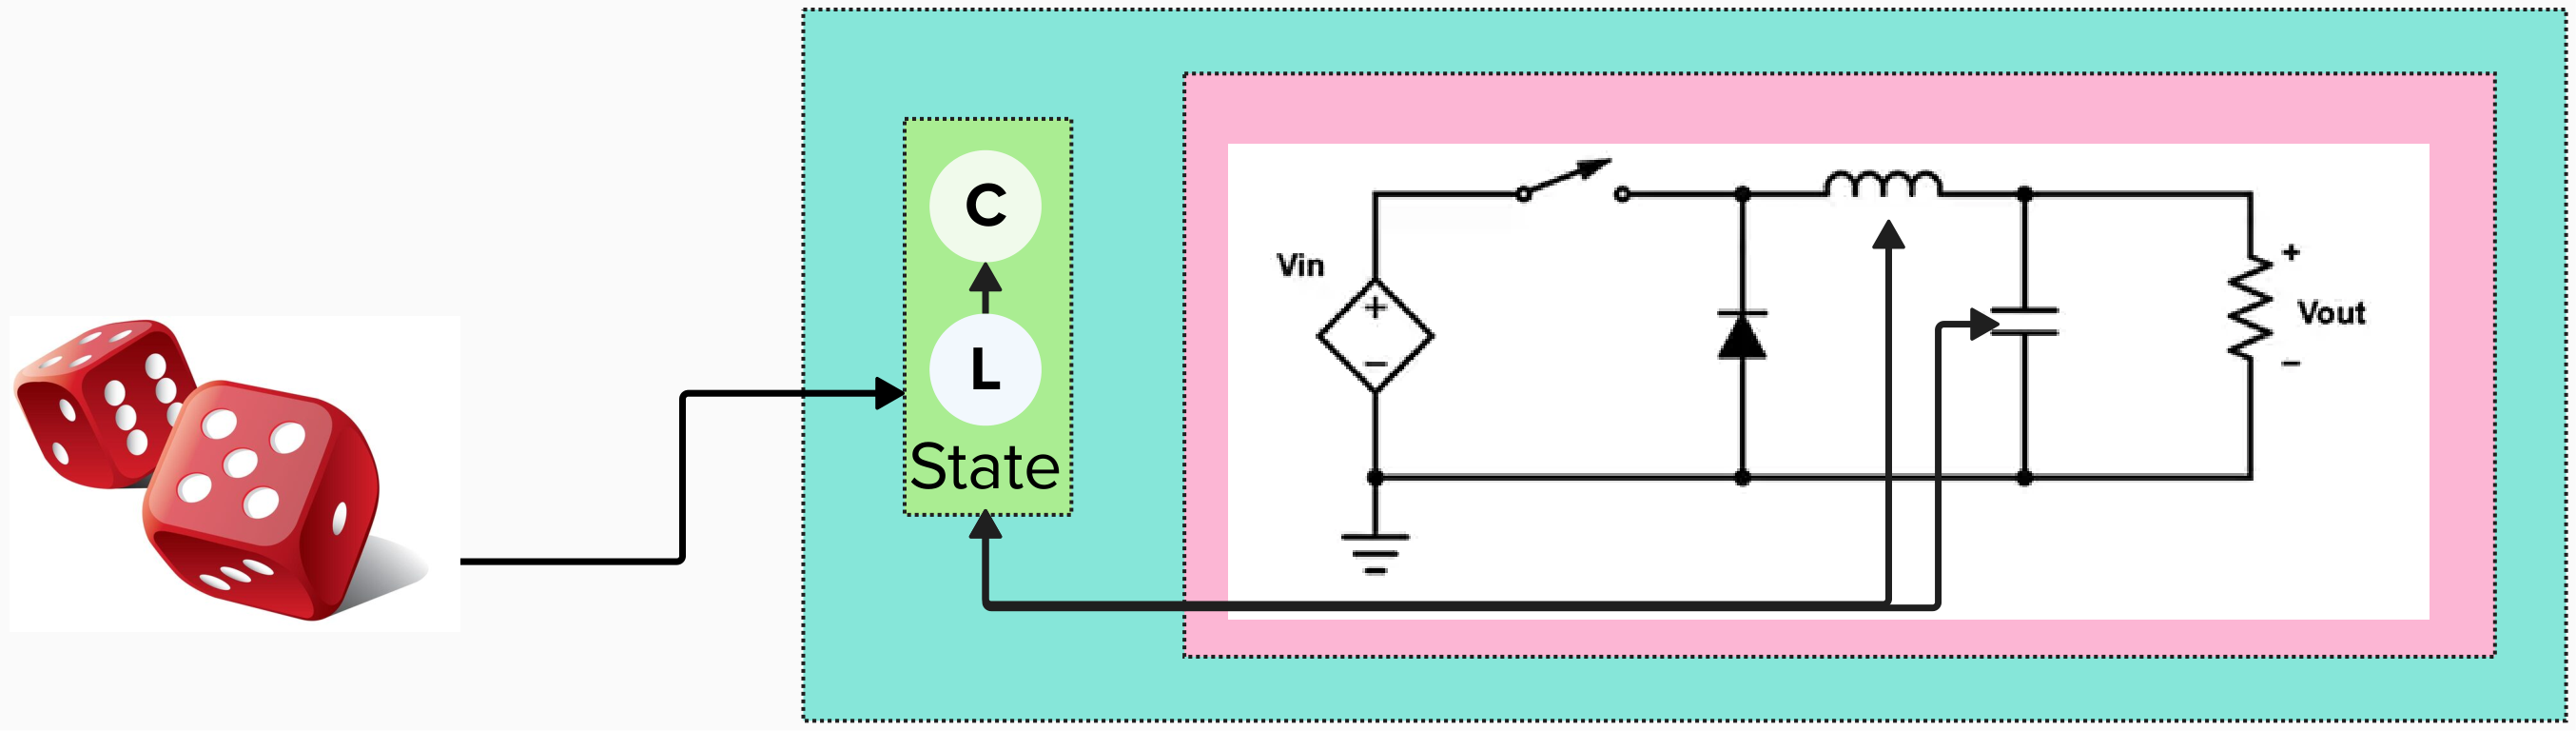
\includegraphics[width=0.7\textwidth]{3Experiment/2Experiment/1Random_Set_State.png}
\caption{Visualisierung der Zustandsgenerierung mit dem Würfel und die Setzung der Werte in der DCDC-Schaltung.}
\label{fig:state_generation}
\end{figure}

% \subsection{Makrozyklus Schritt 2: Entscheidungsfindung durch den Actor}

Nachdem der initiale Schaltungszustand durch eine Zufallsverteilung generiert wurde, kommt der Actor ins Spiel, der auf Basis der aktuellen Kapazitäts- (C) und Induktivitätswerte (L) Entscheidungen trifft. Der Actor, ein wesentlicher Bestandteil des Reinforcement Learning Systems, ist eine komplexe Funktion, die sich aus mehreren Gewichtungen (weights) und Verzerrungen (biases) zusammensetzt. Diese werden im Laufe des Vorwärtsdurchlaufs (Forward Propagation \ref{sec: Forward Propagation}) durch das Netzwerk multipliziert und summiert.

\begin{itemize}
		\item Innerhalb des Actors wird die Eingabe durch jede Schicht des neuronalen Netzwerks transformiert, wobei nach jedem Schichtdurchgang eine nicht-lineare Aktivierungsfunktion \ref{eq:activation_function} angewandt wird, um die Linearität der Operationen zu durchbrechen.
		\item Im spezifischen Kontext unseres Systems ist die Aktivierungsfunktion der letzten Schicht eine  Hyperbelfunktion (tanh), die die Ausgabe des Netzwerks beeinflusst und zu einem komplexen, nicht-linearen Ergebnis führt.
\end{itemize}

Die Ausgabe des Actors sind die PID-Werte, die für die Steuerung des nächsten Schrittes im System verwendet werden. Diese Werte sind das Resultat des durch die tanh-Funktion modifizierten Outputs und stellen somit eine fein abgestimmte Reaktion auf den Zustand der Schaltung dar. Diese Werte werden anschließend skaliert, um realistische PID-Reglerparameter zu erhalten:

\begin{itemize}
	\item Der Proportionalwert (Kp) wird zwischen 0 und 10 skaliert.
	\item Der Integralwert (Ki) wird zwischen 0 und 1 skaliert.
	\item Der Differentialwert (Kd) wird zwischen 0 und 0.1 skaliert.
\end{itemize}

Diese Skalierung ist entscheidend, um die Ausgangswerte des neuronalen Netzes in praktikable Steuerparameter zu überführen. Die Transformation gewährleistet, dass die PID-Werte in einem Bereich liegen, der für die Regelung des Systems adäquat ist und reflektiert die praktischen Anforderungen an die Systemsteuerung. 


\begin{figure}[htbp]
\centering
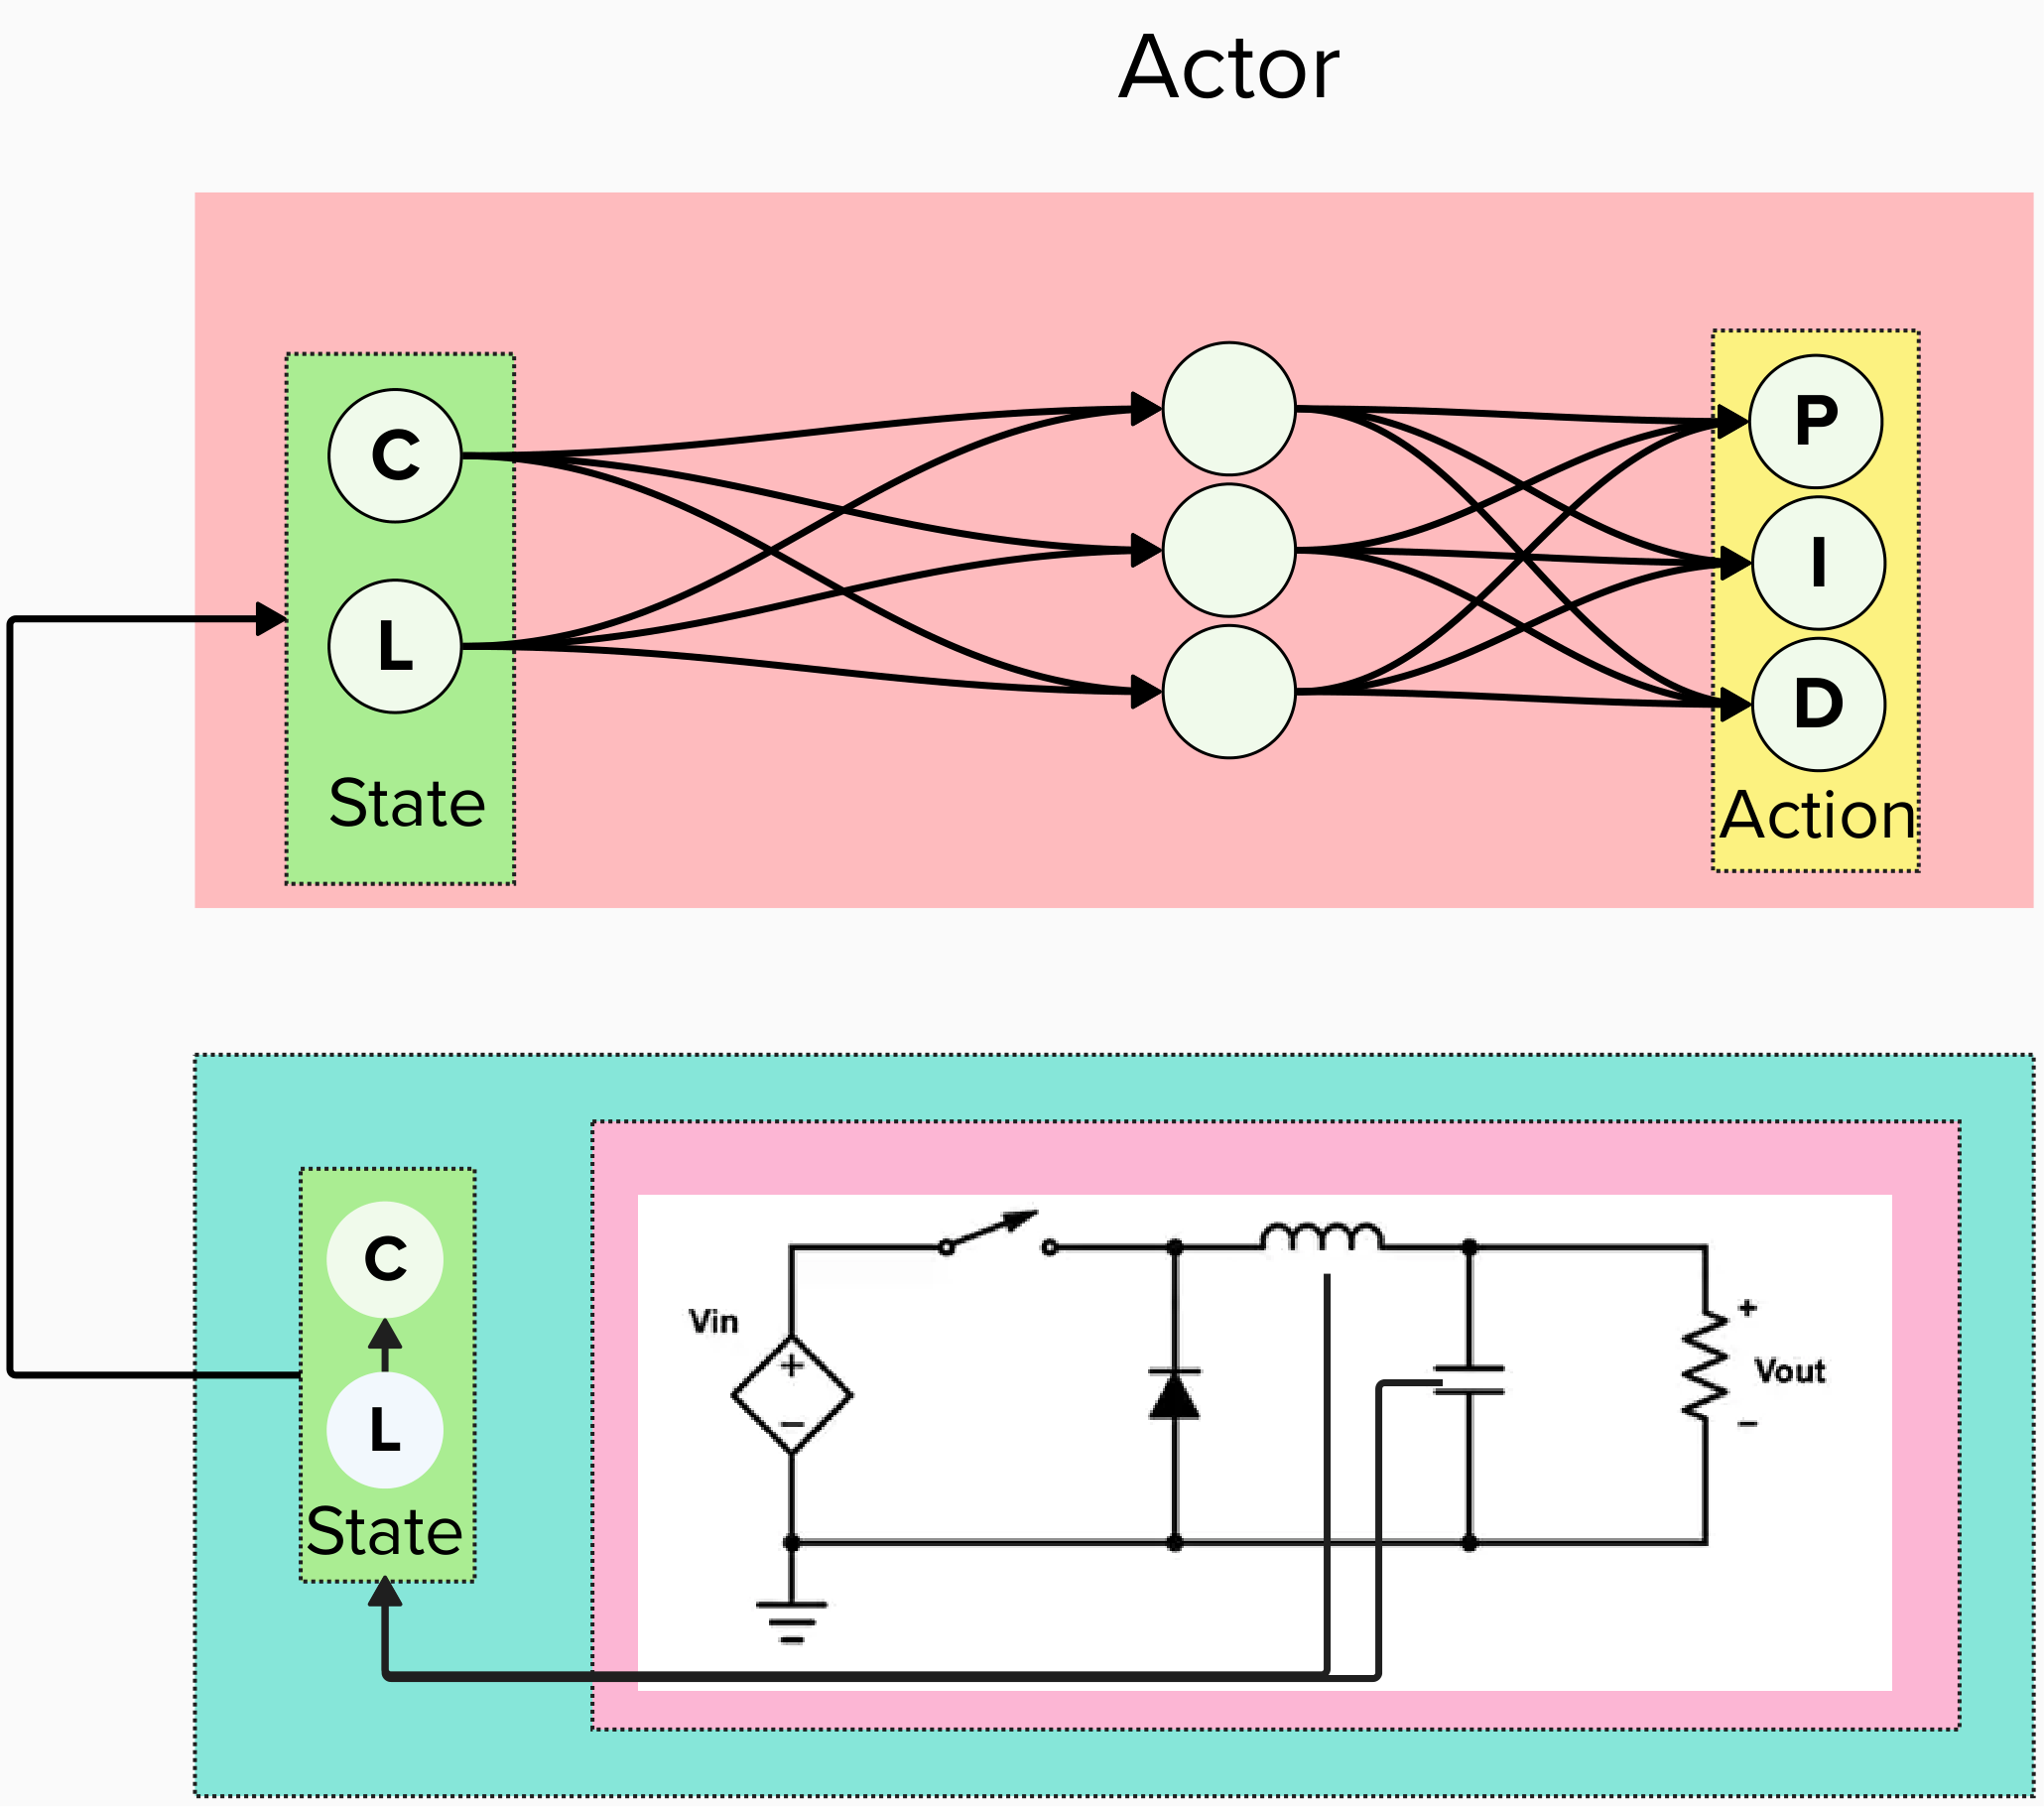
\includegraphics[width=0.5\textwidth]{3Experiment/2Experiment/2Actor.png}
\caption{Die Forward Propagation im Actor-Modul, die den Zustand S (C, L) aufnimmt und über ein mehrschichtiges neuronales Netzwerk PID-Aktionswerte ausgibt.}
\label{fig:actor_decision_making}
\end{figure}




\label{sec:Results_Presentation}

Nach der erfolgreichen  Realisierung einer robusten Actor-Critic-Architektur haben wir eine entscheidende Phase erreicht: die Präsentation unserer Forschungsergebnisse. Anfänglich zeigte unser Modell vielversprechende Resultate mit scheinbarer Leichtigkeit. Allerdings stellten wir fest, dass eine weitere Verfeinerung notwendig war, um exzellente Leistungswerte zu erzielen. Diese kontinuierliche Verbesserung war besonders im Feintuning-Prozess bemerkbar, wenngleich die Qualität der Ergebnisse anfangs unsicher war.

Um die Validität unserer Ergebnisse zu überprüfen, griffen wir auf Bayesian Optimization zurück, eine Technik, die für ihre herausragende Fähigkeit zur Auffindung optimaler Parameterwerte bekannt ist. Das Modell wurde speziell so konzipiert, dass es mit dieser Technik kompatibel ist.

Mit Bayesian Optimization konnten wir gezielt spezifischen Degradationszustand auswählen und diesen als Benchmark heranziehen. Diese gezielte Auswahl ermöglichte es uns, die Effektivität und Genauigkeit der Architektur zu bestätigen.

Abbildung \ref{fig:Bayesian_PID_Optimization} zeigt eine dreidimensionale Visualisierung verschiedener PID-Konfigurationen, die durch Bayesian Optimization ermittelt wurden. Die verschiedenen Farbnuancen korrespondieren mit den erzielten Rewards, wobei dunklere Farbtöne höhere Belohnungen symbolisieren. Die systematische und gleichmäßige Abtastung des Parameterraums durch Bayesian Optimization ist deutlich zu erkennen. Die Intensivierung der Suche in Bereichen, die vielversprechende Werte zeigten, verdeutlicht die zielgerichtete und effiziente Natur des Optimierungsprozesses.

\begin{figure}[h]
\centering
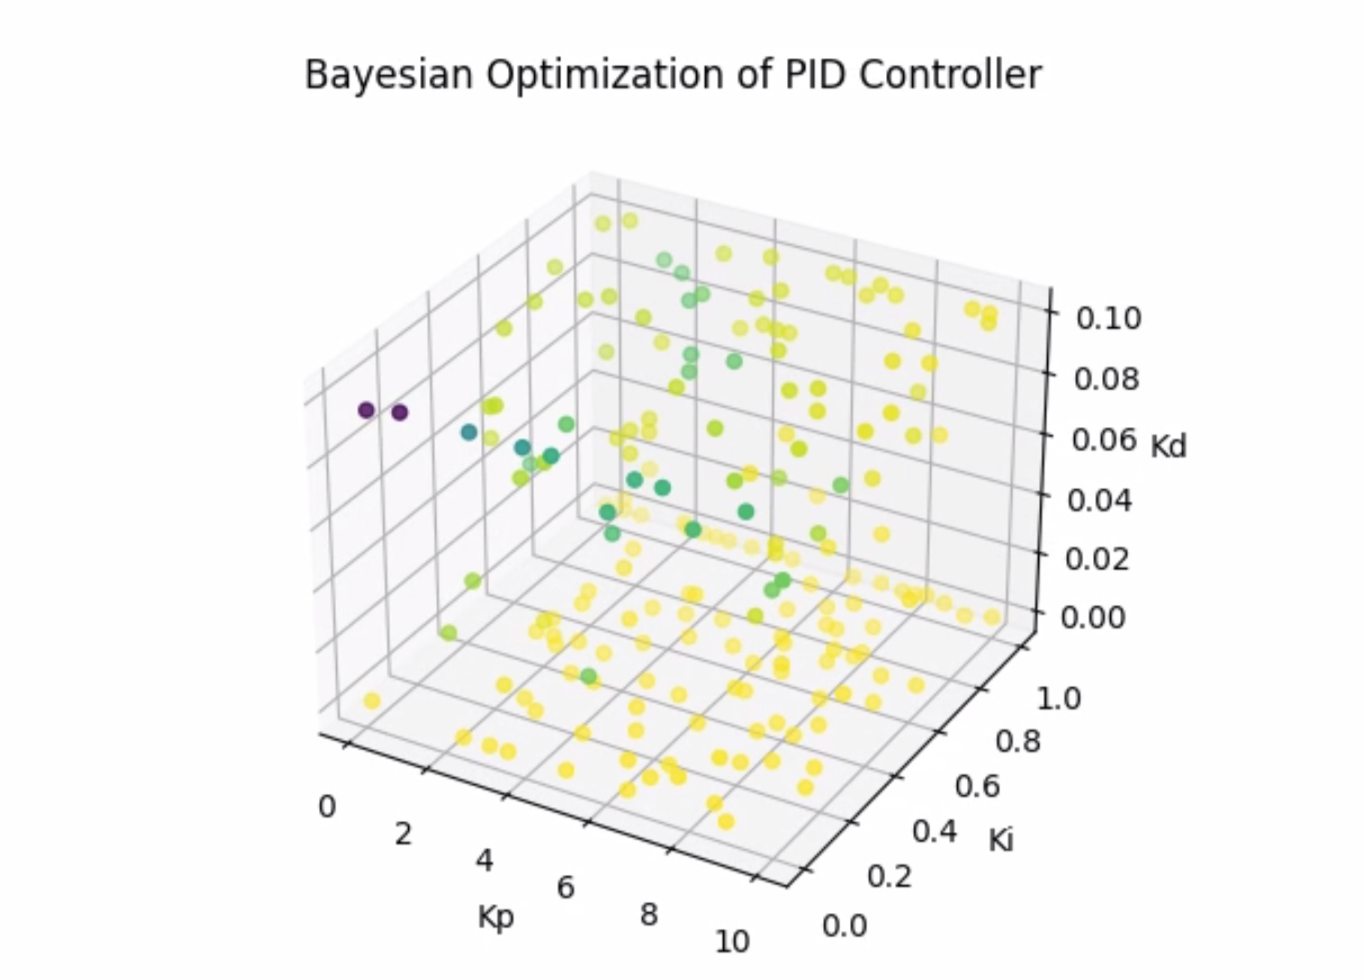
\includegraphics[width=0.6\textwidth]{4Ergebnisse/0Bayes_ergebnisse.png}
\caption{Dreidimensionale Darstellung der Bayesian Optimization von PID-Controller-Parametern.}
\label{fig:Bayesian_PID_Optimization}
\end{figure}

Die Präzision dieser Optimierungsmethode ermöglichte es uns, einen Referenzwert für die Regelungsleistung zu etablieren. Dieser Wert wurde anschließend als Benchmark für das manuelle Feintuning der Hyperparameter unserer Regelung verwendet.

